\begin{figure}[H]
  \centering
  \begin{minipage}[b]{0.3\linewidth}
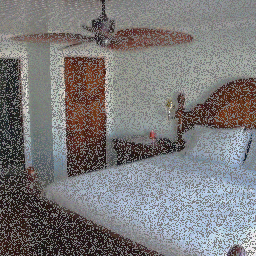
\includegraphics[width=\linewidth]{Picture/input/00008.png}
    \caption{加噪图像6}
    \label{noised image }
  \end{minipage}
  \hspace{0.1cm} % Space between images
   \begin{minipage}[b]{0.3\linewidth}
    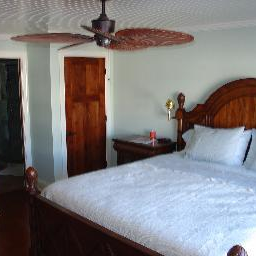
\includegraphics[width=\linewidth]{Picture/label/00008.png}
    \caption{原始图像6}
    \label{original image }
  \end{minipage}
\hspace{0.1cm}
  \begin{minipage}[b]{0.3\linewidth}
    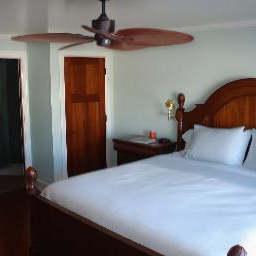
\includegraphics[width=\linewidth]{Picture/recon/00008.png}
    \caption{还原图像6}
    \label{inpainted image}
  \end{minipage}
  \label{整块损坏图像}
\end{figure}